\Chapter{THE APPROACH AND STUDY DEFINITION}\label{sec:Theme1}

%TOTAL = 15 pages

\section{The Approach}

%2 pages

This section will describe the steps followed to design \ac{TEDIOUS}, our proposed machine learning detector to identify design technical debts to self-admit. It will also define its characteristics, how it works and how to use it. \ac{TEDIOUS} works at method-level since it is typically the granularity at which developers introduce \ac{SATD}, as proven by \citet{MaldonadoS15} and \citet{PotdarS14}. In other terms, it is able to define whether a method contains a design technical debt or not. Class-level granularity would be to coarse because technical debts normally admitted by developers are related to specific and punctual issues in the source code. Additionally, a class could contain a \ac{TD} but it would be impossible to precisely identify the source of the problem since a class contains several methods and \ac{LOC}. \par 

\begin{figure}[t]
	\centering
	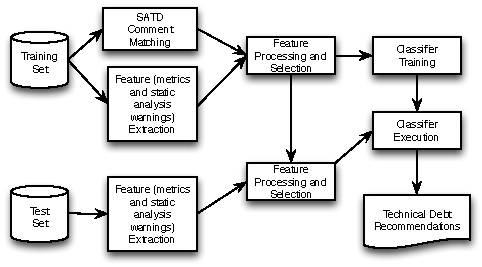
\includegraphics[width=\linewidth]{figs/approach.pdf}
	\caption{Proposed approach for recommending SATD.}
	\label{fig:approach}
	\vspace{-4mm}
\end{figure}

\ac{TEDIOUS} works as shown in Figure \ref{fig:approach}. Two datasets are required as inputs: the training set and the test set. The training set contains labeled data, which his source code from a project where technical debts are known and have been self-admitted through comments. The test set contains unlabeled data, which can be any source code under development or already released where \ac{TEDIOUS} can attempt to recommend where \ac{TD} should be self-admitted or where source code should be improved. \par 
	
For the training set, various kinds of metrics and static analysis warnings are extracted from the source code as well as \ac{SATD} methods in order to build an oracle to train the model. These labeled \ac{SATD} methods are essential for the machine learner since supervised learning is performed, meaning each method is labeled as true or false. It is true when the method is a \ac{TD} and false if it is not. \par 

Once all the information is extracted, feature preprocessing and selection is applied. Multi-collinearity, a phenomenon occurring when two predictor variables are highly correlated, meaning that one can be linearly predicted by the other, is dealt with. Feature selection is applied to retain only the most relevant variables to train the predictor. Finally, re-balancing is performed to address the issue of the low amount of positive examples, \textit{i.e.} \ac{SATD} methods. With the preprocessed features and the oracle now defined (each method is labeled as \ac{SATD} or not), the machine learners can be trained. \par 

In parallel, the test set is also being prepared. The same features are extracted from the source code but no \ac{SATD} matching is required since the data is unlabeled. \ac{SATD} are only required for the oracle, which is used for training the models. A similar feature filtering is applied, except for the re-balancing since it is only required on the labeled data. With both the test set and the previously trained classifier, predictions can be made on the test set in order to recommend when to self-admit technical debts.

\subsection{Features}

3 pages

\subsection{Identification of Self-Admitted Technical Debt}

0.5 page

\subsection{Feature Preprocessing}

3 pages

\subsection{Building and Applying Machine Learning Models}

0.5 page
	
\section{Study Definition}

0.5 page

\subsection{Dataset}

2 pages

\subsection{Analysis Method}

3.5 pages